%Nama Kelompok: Sistem_Operasi_Deadlock
%Kelas: D4 TI 1B
%Alit Fajar Kurniawan(1174057) 
%Muhammad Iqbal Panggabean(1174063)
%Muhammad Afra Faris(1174041)
%Khadijah Hasanah Puteri Harahap(1174044)

\section {matplotlib untuk plot dari arduino}

\subsection {Matplotlib}
\subsubsection {Pengertian Matplotlib}
	Pengertian Matplotlib merupakan librari plotting 2D phyton yang dapat menghasilkan gambar publikasi yang bagus dalambentuk berbagai format perangkat keras dan lingkungan yang interaktif sepanjang platform. Matplotib juga dapat dimanfaatkan didalam script python, iphyton dan shell phyton. matplotib juga berusaha utnuk dapat menjadikan hal yang mudah akan menjadi hal yang lebih mudah, dan bisa jadi hal yang sulit menjadi hal yang lebih sulit bahkan sangat.
	
\subsection {Menginstall Matplotlib}
	Untuk instal matplotlib caranya sangat sederhana dan sangat mudah. Saat ini saya berkerja sama dengan Mac OS X, sehingga saya dapat akan menampilkan bagaimana muntuk install librari pada operasi system itu. Silahkan lihat halaman instalasi matplotlib.	Matplotib dapat diinstall dengan cara yaitu menjalankan beberapa perintah berikut ini didalam terminal. biasanya kebanyak orang menggunakan pip, tetapi bisa juga untuk menggunakan beberapa tool lainnya.

	\subsubsection{cara install}
	\begin{verbatim} 
	
		curl -O https://bootstrap.pypa.io/get-pip.py
		python get-pip.py
		pip install matplotlib

	\end{verbatim}
	
\subsection {Gambar plot dasar matplotlib}
	\begin{figure}[ht]
	\centerline{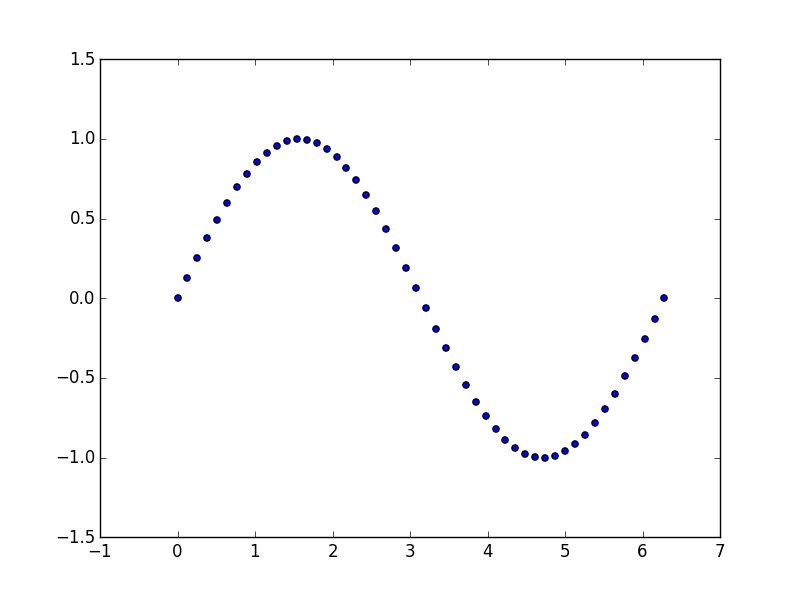
\includegraphics[width=1\textwidth]{figures/matplotib.JPEG}}
	\caption{plot dasar matplotlib}
	\label{Gambar}
	\end{figure}
      
      Gambar \ref{Gambar} Contoh gambar plot dasar matplotlib.
	  
\subsection {Dua tipe plot}
\begin{enumerate}
\item 
	1. Plot Garis
		Dalam hal ini, menggunakan matplotlib. pyplot, yang menyajikan framework plotting seperti MATLAB. dalam artian lain, menyajikan sebuah koleksi function bergaya command yang membuat matplotlib berkerja layaknya seperti MATLAB.
\item
	2. Plot Sebaran
		Plot sebaran merupakan grafik yang menampilkan relasi antara dua set data, seperti relasi antara tinggi dan umur.
\end{enumerate}
	  
	  
